\section{Hosting}

Both the backend and frontend were hosted on Render. I chose Render as a good
low cost option for hosting the web service as it offers a free trial period,
constant uptime and backups. A feature I particularly liked was the ability for
the server to instantly deploy whenever I pushed a commit through to github, if
the deployment on render failed then it would revert back to the previous
instance meaning the website was never down. 

I have two servers with render, one handles the database and the other runs the
backend and frontend. The database server has 256 MB of RAM; 0.1 share of a CPU
and 1 GB of storage. A single instance of a Postgres database is available on
this service - which is free for the first 30 days and then costs \$5 a month.
Meanwhile the backend and frontend instance are run with 512MB of ram and a 0.5
share of a CPU with no storage as all permanent data is held on the database.
This second service costs \$7 for a cost of about £10. These resources should be
sufficient for this project as only small amounts of data are involved.
Eventually, I aim to migrate the website to a university hosted server to reduce
the cost to \pounds10.

\section{Backend}

\subsection{postgreSQL database}

\begin{figure}[H]
    \centering
    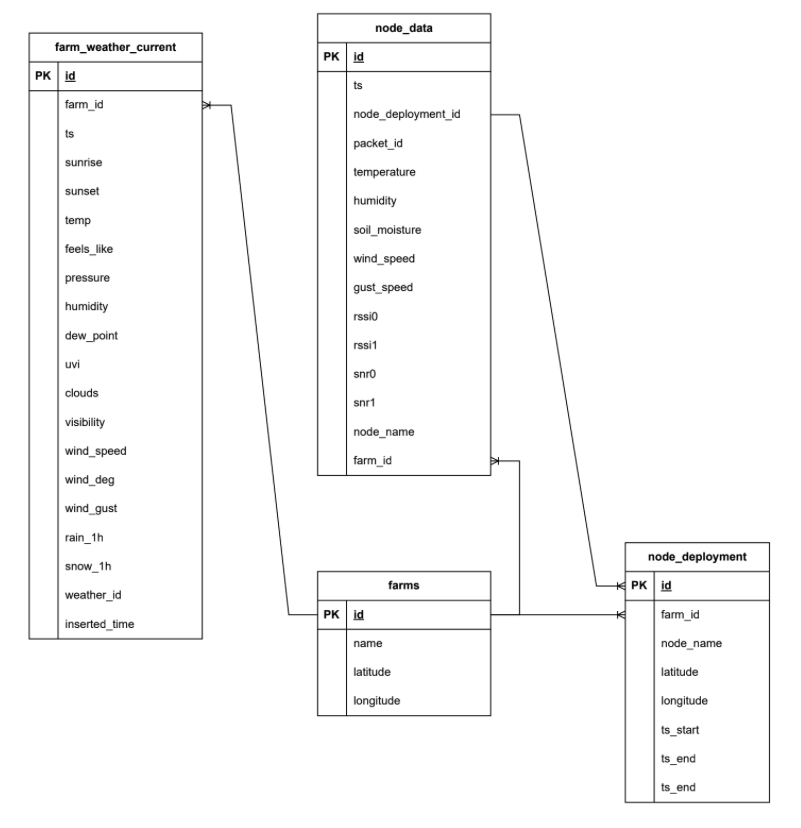
\includegraphics[width=0.8\textwidth]{contents/part-3/fig3/postgres_diagram.png}
    \caption{Table schema for postgreSQL database}
    \label{fig:db_schema}
\end{figure}

The database has four tables:

\begin{itemize}     
      \item farms: this holds a list of where the nodes are (or have been)
      deployed. The longitude and latitude of the farm is then used in API calls
      to OpenWeather (more on this below) which is used to fetch current and
      forecasted weather data.
      \item node\_deployment - This holds the precise longitude and latitude of
      each node as well as information on when the deployment started and ended.
      If the nodes are moved then this table is updated with new information.     
      \item node\_data - Holds the full set of readings from each node.    
      \item farm\_weather\_current - Holds current weather information from API
      calls to OpenWeather taken every 10 minutes and is strictly used to train
      the machine model explained in the machine learning section.
 \end{itemize} 


\subsection{Building an API}

With the database configured, I then developed a backend API using TypeScript,
Node.js, and express. This service is responsible for interpreting incoming HTTP
requests and performing corresponding database operations - it is essentially
the bridge between the gateway hardware and the database. In addition to
handling sensor data, the service also integrates with an external weather API
in order to retrieve both current conditions and forecast data, which are then
stored alongside the locally collected sensor readings as explained above.

The API inserts data into the database when it receives a POST request. The body
of the POST request contains a JSON body which is parsed, processed and added to
the database by the API. Data can be retrieved for display by the frontend using
a GET request.

The entire api is written using Typescript. Typescript is javascript with added
syntax that forces strong typing and features to enable error catching earlier
on. When typescript is compiled it produces a javascript file which contains the
actual code that is then executed. The main benefit of typescript is that it
leads to much more robust code with vastly fewer typing errors that vanilla
javascript can often let slip by. As I needed my API to have constant up time
and reliably insert and select from my database this made typescript ideal for
this application.

On top of TypeScript I used Node.js and the Express framework. Node.js allows
JavaScript to run on the server instead of inside a client browser, which lets
the project share a single language (i.e. JavaScript) across frontend and
backend development. It is well suited to creating APIs that handle many
simultaneous HTTP requests while calling on external APIs. This is because Node
runs asynchronously: when slow database queries are being executed Node will
continue listening and processing further requests. This non-blocking behaviour
means Node can handle large numbers of concurrent requests at the same time.
Additionally the node packet manager (called with npm) has a large set of useful
libraries and allows my project to be rapidly set up on new computers without
having to retrieve required packages from different sources.

Express is a framework specific to Node.js that gives useful tools for creating
the API endpoints. I used express to write my request-handling functions for
each URL endpoint. These functions process incoming HTTP requests to the
endpoint and then execute the SQL query associated with that endpoint. Instead
of constantly opening new connections with the database I used the pg.Pool
library to pool requests together on the same connection. This helped to improve
the speed of SQL lookups and inserts helping requests to be executed faster,
which in turn improved the perceived performance of the webapp.

\subsection{Security}

Security was important in the design of the backend API as the end points are
exposed to the internet and thus any internet connected device is able to call
these. Therefore I had to take steps to prevent erroneous calls (such as from
bots) to my API endpoints which could insert data incorrectly or scrape the
contents.

The first step I took was to use environment variables inside Render to hide
sensitive information such as API keys and passwords. These variables are hidden
from any source documents served to the browser and are injected separately at
deploy time. This prevents the information from leaking into the public domain.

Then I needed to prevent any unauthorised machine attempting to perform API
calls on my backend. The approach I took to this was to follow guidelines set
out in RFC 6750 related to the use of 'Bearer tokens' (essentially a password
check) \cite{rfc6750}. For this I checked that all incoming HTTP requests to my
API had an 'Authorization' line in their headers. I then checked whether the
string token after this matched the SECRET\_WORD variable in my environment
variables. Any request to the database without the correct header and token is
automatically rejected.

Finally in case those security measures are not sufficient and a malicious actor
gets access to my API end points I then added protections against SQL
injections. SQL injections are a technique where an attacker can try to
manipulate a database by sending a crafted input that alters the intended
purpose of the endpoint.

For example if my API end point was designed to allow selections from a database
it might naïvely allow queries such as this:

\verb|SELECT ${httpBody.column} FROM ${httpBody.table_name};|

Expecting the \verb|httpBody| to contain a JSON with \texttt{column = "*"} and
\texttt{table\_name = "node\_data"}, for instance. 

However, if someone were to name their column as \texttt{"*"} and their
table\_name as \texttt{"node\_data; DROP TABLE node\_data;"} the effective command
would change to:

\verb|SELECT * FROM node_data; DROP TABLE node_data;|

This command would then select the data as intended before completely destroying
the table and all of its data. To prevent this from happening I whitelisted
valid table\_names like so (psuedo-code for clarity);

\begin{verbatim}
const white_listed_tables = new Set('node_data');

if (!white_listed_tables.has(httpBody.table_name)) {
    return 404 error;
}
\end{verbatim}



\subsection{Weather API integration}

The weather API I settled on using to help build data for the forecasting
function of the webapp was the One Call API 3.0 by OpenWeather. This API offers
current weather data at a 10 minute resolution as well as 48 hour ahead hourly
and 8 day ahead daily weather forecasts. The API permits up to 1000 calls per
day before separate payment is required. As I would only be requesting one
current weather data reading and one forecast data reading on 10 minute
intervals I would only put through 288 requests per day which is well within the
free limits.

To set up automatic API retrieval from my backend to the weather API I used the
node-cron library to set up a 10 minute job on my host server. This then called
related functions to get both current and forecasted data for use with my
machine learning model.

\section{Frontend webapp}

The frontend of my project is written in HTML, CSS and Javascript, which is an
archetypal web development stack.

\subsection{picoCSS}

picoCSS is the library I used for the default styling of my webapp. I liked its
minimal and low distraction look which I thought was ideal for presenting data.
It also had good mobile to desktop scaling which meant my webapp (at least the
non-chart parts) worked on mobile and desktop with little work needed.

\subsection{Apache echarts}

Apache echarts is a javascript library that I have used to build the charts for
my webapp. Data for charts is fetched from the backend and then loaded into a
'series' object. Apache echarts then renders the data series onto a graph with a
variety of options that I have chosen to improve data clarity.

\subsection{Making the app mobile friendly}

I wanted the webapp to be accessible for both desktop and mobile users. What
tends to make this difficult is the fact that scaling on desktop and mobile is
normally very different. Mobile devices have a longer vertical axis while on
desktop it tends to be the reverse - so I needed to ensure elements were
reactive to the screen size of the viewer.

picoCSS comes with much of this reactive formatting as standard on default HTML
elements (selection boxes, divs, titles, navigation bars etc). However
integrating echarts was difficult as picoCSS styles cannot directly apply to
this. I therefore took actions to improve the usability for mobile users, as
summarised below:

\begin{enumerate}
    \item Dynamic tooltip: The webapp can tell if the viewer is a touch screen
          and if so it will make the tool tip hover slightly away from the point
          of touch. While on desktop the user will want to hover over a
          datapoint and see the tool tip appear where they are hovering, on
          mobile the digit used to select may cover important tooltip
          information. By making sure the tooltip hovers slightly away from the
          selection this is no longer a problem.
    \item Dynamic chart and font size: Echarts comes with no standard method of
          resizing chart data depending on the size of the device viewing the
          chart. Therefore I developed a number of functions to improve
          readability on mobile devices by dynamically decreasing chart height
          and font size for mobile screen sizes.
    \item
\end{enumerate}

\subsection{ Walkthrough of features}

Walkthrough of main features with images and 



